\documentclass[12pt,a4paper]{article}
\usepackage[utf8]{inputenc}
\usepackage{geometry}
\usepackage{tikz}
\usepackage{xcolor}
\usepackage{graphicx}
\usepackage{titlesec}
\usepackage{fancyhdr}
\usepackage{tcolorbox}
\usepackage{enumitem}
\usepackage{pgfplots}
\pgfplotsset{compat=1.18}

% Font packages - Choose ONE of these options:
% \usepackage{helvet} % Option 1: Helvetica (sans-serif)
\renewcommand{\familydefault}{\sfdefault} % Use sans-serif font as default

% Uncomment just ONE of these font alternatives if you want to try them:
% \usepackage{tgpagella} % Option 2: TeX Gyre Pagella (similar to Palatino)
% \usepackage{bookman} % Option 3: Bookman
% \usepackage{tgheros} % Option 4: TeX Gyre Heros (similar to Helvetica but enhanced)
% \usepackage{lmodern} % Option 5: Latin Modern 
% \usepackage{libertine} % Option 6: Linux Libertine (elegant serif)
\usepackage{mathpazo} % Option 7: Palatino
% \usepackage{charter} % Option 8: Charter

% Define colors
\definecolor{hydrosensblue}{RGB}{37, 51, 114}
\definecolor{hydrosenscyan}{RGB}{81, 186, 215}

% Page setup
\geometry{
    top=2cm,
    bottom=2cm,
    left=2cm,
    right=2cm
}

% Set up fancy headers
\pagestyle{fancy}
\fancyhead{}
\fancyfoot{}
\renewcommand{\headrulewidth}{0pt}
\renewcommand{\footrulewidth}{0pt}

% Title formatting
\titleformat{\section}
  {\normalfont\Large\bfseries\color{hydrosensblue}}
  {}
  {0em}
  {}[\titlerule]

\titleformat{\subsection}
  {\normalfont\large\bfseries\color{hydrosensblue}}
  {}
  {0em}
  {}

% Document begin
\begin{document}

% First page (cover)
\begin{titlepage}
    \textbf{\Huge \color{hydrosensblue}{RSS}}
    
    \vspace{0.5cm}
    
    \textbf{\huge \color{hydrosensblue}{HYDROSENS}}
    
    \vspace{0.5cm}
    
    \textbf{\Large{ENVIRONMENTAL MONITORING REPORT}}
    
    \vspace{1cm}
    
    \vspace{1cm}
    
    \textbf{\Large{REGION : \quad Name\_ABALOU Abla - Autre parcelle}}
    
    \vspace{0.5cm}
    
    \textbf{\Large{TIME PERIOD : \quad 23 DEC 2024 - 27 JAN 2025}}
\end{titlepage}

\newpage

% Overview page
\section*{OVERVIEW}

\begin{minipage}{\textwidth}
This report analyzes environmental conditions in Name\_ABALOU Abla - Autre parcelle from December 23, 2024, to January 27, 2025. The analysis includes NDVI, vegetation fraction, soil fraction, precipitation, temperature, and curve number. The data indicates moderate vegetation health with negligible rainfall and stable temperature, suggesting a need for water management strategies and soil conservation practices.
\end{minipage}

\vspace{1cm}

\begin{tcolorbox}[title={\textbf{KEY INSIGHTS}}, colback=white, colframe=hydrosensblue]
\begin{enumerate}[label=\textbf{\arabic*.}, leftmargin=1.5em]
    \item \textbf{Moderate Vegetation Health}\\
    NDVI values indicate moderate vegetation density with a slight fluctuation observed over the period.
    \item \textbf{Negligible Rainfall}\\
    Precipitation remained virtually zero throughout the reporting period, which might stress the vegetation.
    \item \textbf{Stable Temperature}\\
    Temperature remained relatively constant, which can be good for stable crop developement if water demand is satisfied.
    \item \textbf{High vegetation cover fraction}\\
    Vegetation fraction is high (above 0.75) suggesting dense vegetation cover
\end{enumerate}
\end{tcolorbox}

% Metric pages

\newpage

\section*{NORMALIZED DIFFERENCE VEGETATION INDEX}
\textit{Indicates vegetation health from 0 to 1.}

\vspace{0.5cm}

\parbox{\textwidth}{ % Keep this parbox for horizontal layout
    \begin{minipage}[t]{0.48\textwidth}
        \vspace{0.3cm}
        \textbf{\Large{0.36}}
        \vspace{0.3cm}
        \textbf{MEAN VALUE}\\
        An average NDVI of 0.36 suggests moderate vegetation density for Name\_ABALOU Abla - Autre parcelle, indicating some vegetative activity but potentially below optimal levels.
        \vspace{0.5cm}

        \textbf{TIME SERIES INSIGHT}\\
        NDVI values fluctuated between 0.29 and 0.43 during the reporting period. There was an increase in NDVI in early January, followed by a gradual decline towards the end of January, suggesting a potential response to environmental conditions or management practices.
    \end{minipage}\hfill
    \begin{minipage}[t]{0.48\textwidth}
        \begin{center}
            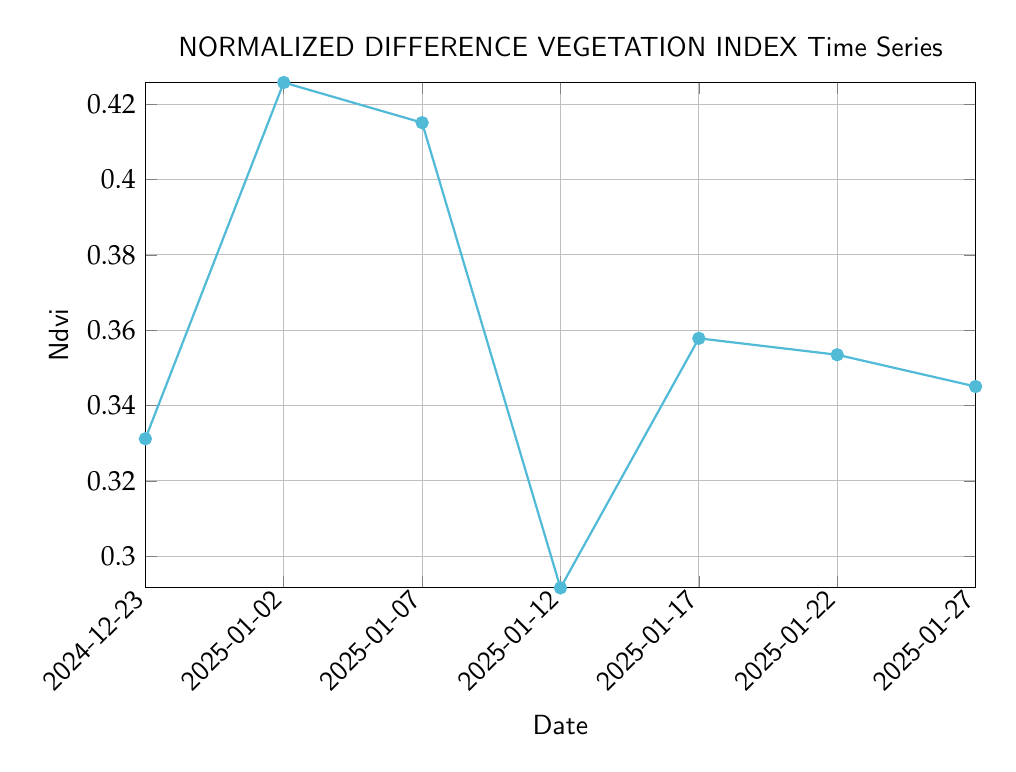
\begin{tikzpicture}
            \begin{axis}[
                width=\linewidth,
                height=8cm,
                xlabel={Date},
                ylabel={Ndvi},
                xmin=1, xmax=7,
                % Use xtick=data to let pgfplots figure out ticks from xticklabels
                xtick=data,
                xticklabels={ % Use a join filter to ensure no trailing commas or extra spaces
                    2024-12-23, 2025-01-02, 2025-01-07, 2025-01-12, 2025-01-17, 2025-01-22, 2025-01-27
                },
                title={NORMALIZED DIFFERENCE VEGETATION INDEX Time Series},
                grid=both,
                xticklabel style={rotate=45,anchor=east},
                enlargelimits=false,
                % Add "unbounded coords=jump" to handle potential non-numeric data gracefully
                unbounded coords=jump
            ]
            \addplot[
                color=hydrosenscyan,
                mark=*,
                thick,
            ]
            coordinates {
                % Safely generate coordinates on a single line
                    % Ensure y_val is numeric and not empty/None.
                    % If it could be missing, you might need a conditional check here
                    % e.g., 
                    (1, 0.3311726052982869) % Use 'nan' for missing values
                    % Ensure y_val is numeric and not empty/None.
                    % If it could be missing, you might need a conditional check here
                    % e.g., 
                    (2, 0.4257457384621265) % Use 'nan' for missing values
                    % Ensure y_val is numeric and not empty/None.
                    % If it could be missing, you might need a conditional check here
                    % e.g., 
                    (3, 0.4150797399130213) % Use 'nan' for missing values
                    % Ensure y_val is numeric and not empty/None.
                    % If it could be missing, you might need a conditional check here
                    % e.g., 
                    (4, 0.2915896498347248) % Use 'nan' for missing values
                    % Ensure y_val is numeric and not empty/None.
                    % If it could be missing, you might need a conditional check here
                    % e.g., 
                    (5, 0.35783109319451545) % Use 'nan' for missing values
                    % Ensure y_val is numeric and not empty/None.
                    % If it could be missing, you might need a conditional check here
                    % e.g., 
                    (6, 0.35347229084993753) % Use 'nan' for missing values
                    % Ensure y_val is numeric and not empty/None.
                    % If it could be missing, you might need a conditional check here
                    % e.g., 
                    (7, 0.34504334964796574) % Use 'nan' for missing values
            };
            \end{axis}
            \end{tikzpicture}
        \end{center}
    \end{minipage}%
}\par % Keep this \par immediately after the closing brace of the \parbox
\vspace{1cm}


\newpage

\section*{VEGETATION FRACTION}
\textit{Proportion of ground covered by vegetation.}

\vspace{0.5cm}

\parbox{\textwidth}{ % Keep this parbox for horizontal layout
    \begin{minipage}[t]{0.48\textwidth}
        \vspace{0.3cm}
        \textbf{\Large{0.85}}
        \vspace{0.3cm}
        \textbf{MEAN VALUE}\\
        An average vegetation fraction of 0.85 indicates a high proportion of ground cover by vegetation in Name\_ABALOU Abla - Autre parcelle, suggesting dense vegetation.
        \vspace{0.5cm}

        \textbf{TIME SERIES INSIGHT}\\
        Vegetation fraction remained high throughout the period, ranging from 0.78 to 0.92. There was a peak in mid-January, indicating a period of high vegetation cover, followed by a slight decrease towards the end of the month.
    \end{minipage}\hfill
    \begin{minipage}[t]{0.48\textwidth}
        \begin{center}
            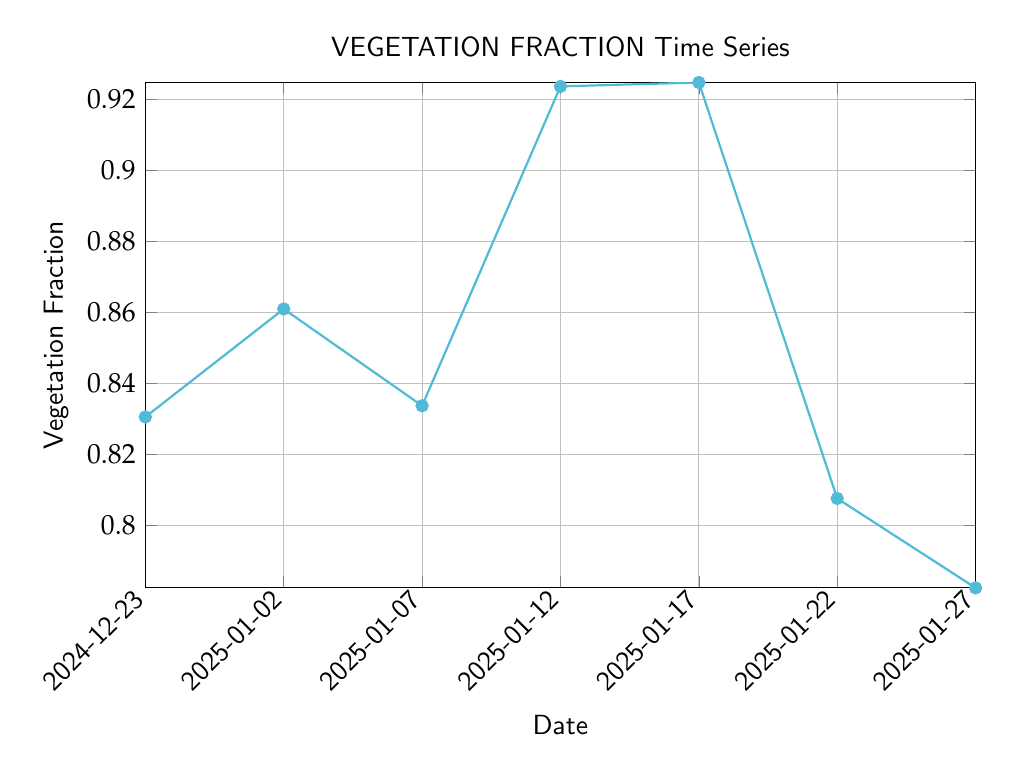
\begin{tikzpicture}
            \begin{axis}[
                width=\linewidth,
                height=8cm,
                xlabel={Date},
                ylabel={Vegetation Fraction},
                xmin=1, xmax=7,
                % Use xtick=data to let pgfplots figure out ticks from xticklabels
                xtick=data,
                xticklabels={ % Use a join filter to ensure no trailing commas or extra spaces
                    2024-12-23, 2025-01-02, 2025-01-07, 2025-01-12, 2025-01-17, 2025-01-22, 2025-01-27
                },
                title={VEGETATION FRACTION Time Series},
                grid=both,
                xticklabel style={rotate=45,anchor=east},
                enlargelimits=false,
                % Add "unbounded coords=jump" to handle potential non-numeric data gracefully
                unbounded coords=jump
            ]
            \addplot[
                color=hydrosenscyan,
                mark=*,
                thick,
            ]
            coordinates {
                % Safely generate coordinates on a single line
                    % Ensure y_val is numeric and not empty/None.
                    % If it could be missing, you might need a conditional check here
                    % e.g., 
                    (1, 0.8305334428763211) % Use 'nan' for missing values
                    % Ensure y_val is numeric and not empty/None.
                    % If it could be missing, you might need a conditional check here
                    % e.g., 
                    (2, 0.8609681717944638) % Use 'nan' for missing values
                    % Ensure y_val is numeric and not empty/None.
                    % If it could be missing, you might need a conditional check here
                    % e.g., 
                    (3, 0.8336931200502222) % Use 'nan' for missing values
                    % Ensure y_val is numeric and not empty/None.
                    % If it could be missing, you might need a conditional check here
                    % e.g., 
                    (4, 0.9236949533177709) % Use 'nan' for missing values
                    % Ensure y_val is numeric and not empty/None.
                    % If it could be missing, you might need a conditional check here
                    % e.g., 
                    (5, 0.9247911147526104) % Use 'nan' for missing values
                    % Ensure y_val is numeric and not empty/None.
                    % If it could be missing, you might need a conditional check here
                    % e.g., 
                    (6, 0.8075661699964561) % Use 'nan' for missing values
                    % Ensure y_val is numeric and not empty/None.
                    % If it could be missing, you might need a conditional check here
                    % e.g., 
                    (7, 0.7823688578321615) % Use 'nan' for missing values
            };
            \end{axis}
            \end{tikzpicture}
        \end{center}
    \end{minipage}%
}\par % Keep this \par immediately after the closing brace of the \parbox
\vspace{1cm}


\newpage

\section*{SOIL FRACTION}
\textit{Volumetric water content in the soil.}

\vspace{0.5cm}

\parbox{\textwidth}{ % Keep this parbox for horizontal layout
    \begin{minipage}[t]{0.48\textwidth}
        \vspace{0.3cm}
        \textbf{\Large{0.11}}
        \vspace{0.3cm}
        \textbf{MEAN VALUE}\\
        The average soil fraction of 0.11 indicates low water content in the soil of Name\_ABALOU Abla - Autre parcelle during the reporting period. This suggests relatively dry soil conditions.
        \vspace{0.5cm}

        \textbf{TIME SERIES INSIGHT}\\
        Soil fraction values fluctuated throughout the period, ranging from approximately 0.03 to 0.21. The soil fraction was relatively low at the beginning of the period, showed a general increase towards the end of the period, indicating a slow gain in the water content. Further monitoring would be needed.
    \end{minipage}\hfill
    \begin{minipage}[t]{0.48\textwidth}
        \begin{center}
            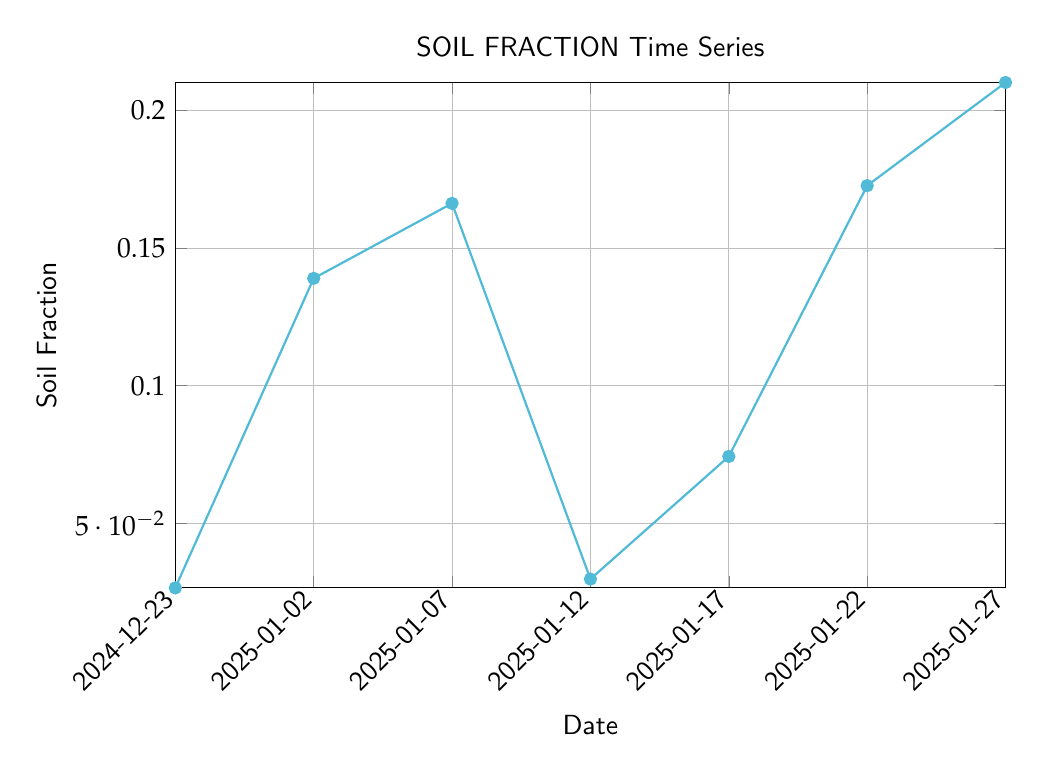
\begin{tikzpicture}
            \begin{axis}[
                width=\linewidth,
                height=8cm,
                xlabel={Date},
                ylabel={Soil Fraction},
                xmin=1, xmax=7,
                % Use xtick=data to let pgfplots figure out ticks from xticklabels
                xtick=data,
                xticklabels={ % Use a join filter to ensure no trailing commas or extra spaces
                    2024-12-23, 2025-01-02, 2025-01-07, 2025-01-12, 2025-01-17, 2025-01-22, 2025-01-27
                },
                title={SOIL FRACTION Time Series},
                grid=both,
                xticklabel style={rotate=45,anchor=east},
                enlargelimits=false,
                % Add "unbounded coords=jump" to handle potential non-numeric data gracefully
                unbounded coords=jump
            ]
            \addplot[
                color=hydrosenscyan,
                mark=*,
                thick,
            ]
            coordinates {
                % Safely generate coordinates on a single line
                    % Ensure y_val is numeric and not empty/None.
                    % If it could be missing, you might need a conditional check here
                    % e.g., 
                    (1, 0.026419354124047587) % Use 'nan' for missing values
                    % Ensure y_val is numeric and not empty/None.
                    % If it could be missing, you might need a conditional check here
                    % e.g., 
                    (2, 0.13903182820553625) % Use 'nan' for missing values
                    % Ensure y_val is numeric and not empty/None.
                    % If it could be missing, you might need a conditional check here
                    % e.g., 
                    (3, 0.1663068799497779) % Use 'nan' for missing values
                    % Ensure y_val is numeric and not empty/None.
                    % If it could be missing, you might need a conditional check here
                    % e.g., 
                    (4, 0.029631506666680928) % Use 'nan' for missing values
                    % Ensure y_val is numeric and not empty/None.
                    % If it could be missing, you might need a conditional check here
                    % e.g., 
                    (5, 0.07423941626975653) % Use 'nan' for missing values
                    % Ensure y_val is numeric and not empty/None.
                    % If it could be missing, you might need a conditional check here
                    % e.g., 
                    (6, 0.172756845036906) % Use 'nan' for missing values
                    % Ensure y_val is numeric and not empty/None.
                    % If it could be missing, you might need a conditional check here
                    % e.g., 
                    (7, 0.21028195963685203) % Use 'nan' for missing values
            };
            \end{axis}
            \end{tikzpicture}
        \end{center}
    \end{minipage}%
}\par % Keep this \par immediately after the closing brace of the \parbox
\vspace{1cm}


\newpage

\section*{PRECIPITATION}
\textit{Amount of rainfall in millimeters.}

\vspace{0.5cm}

\parbox{\textwidth}{ % Keep this parbox for horizontal layout
    \begin{minipage}[t]{0.48\textwidth}
        \vspace{0.3cm}
        \textbf{\Large{0.00}}
        \vspace{0.3cm}
        \textbf{MEAN VALUE}\\
        An average precipitation of 0 mm indicates virtually no rainfall in Name\_ABALOU Abla - Autre parcelle during the reporting period, which may cause dry soil condition.
        \vspace{0.5cm}

        \textbf{TIME SERIES INSIGHT}\\
        Precipitation remained negligible (close to zero) throughout the entire reporting period, indicating very dry conditions. Irrigation strategies might be necessary to sustain vegetation.
    \end{minipage}\hfill
    \begin{minipage}[t]{0.48\textwidth}
        \begin{center}
            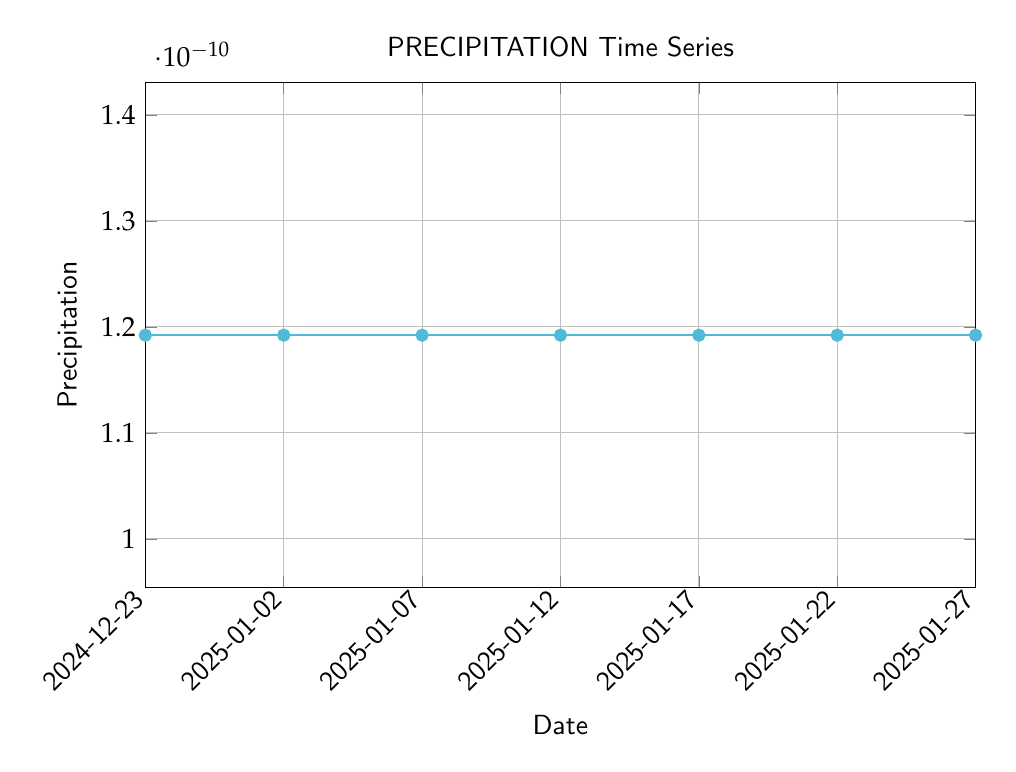
\begin{tikzpicture}
            \begin{axis}[
                width=\linewidth,
                height=8cm,
                xlabel={Date},
                ylabel={Precipitation},
                xmin=1, xmax=7,
                % Use xtick=data to let pgfplots figure out ticks from xticklabels
                xtick=data,
                xticklabels={ % Use a join filter to ensure no trailing commas or extra spaces
                    2024-12-23, 2025-01-02, 2025-01-07, 2025-01-12, 2025-01-17, 2025-01-22, 2025-01-27
                },
                title={PRECIPITATION Time Series},
                grid=both,
                xticklabel style={rotate=45,anchor=east},
                enlargelimits=false,
                % Add "unbounded coords=jump" to handle potential non-numeric data gracefully
                unbounded coords=jump
            ]
            \addplot[
                color=hydrosenscyan,
                mark=*,
                thick,
            ]
            coordinates {
                % Safely generate coordinates on a single line
                    % Ensure y_val is numeric and not empty/None.
                    % If it could be missing, you might need a conditional check here
                    % e.g., 
                    (1, 1.1920928955078125e-10) % Use 'nan' for missing values
                    % Ensure y_val is numeric and not empty/None.
                    % If it could be missing, you might need a conditional check here
                    % e.g., 
                    (2, 1.1920928955078125e-10) % Use 'nan' for missing values
                    % Ensure y_val is numeric and not empty/None.
                    % If it could be missing, you might need a conditional check here
                    % e.g., 
                    (3, 1.1920928955078125e-10) % Use 'nan' for missing values
                    % Ensure y_val is numeric and not empty/None.
                    % If it could be missing, you might need a conditional check here
                    % e.g., 
                    (4, 1.1920928955078125e-10) % Use 'nan' for missing values
                    % Ensure y_val is numeric and not empty/None.
                    % If it could be missing, you might need a conditional check here
                    % e.g., 
                    (5, 1.1920928955078125e-10) % Use 'nan' for missing values
                    % Ensure y_val is numeric and not empty/None.
                    % If it could be missing, you might need a conditional check here
                    % e.g., 
                    (6, 1.1920928955078125e-10) % Use 'nan' for missing values
                    % Ensure y_val is numeric and not empty/None.
                    % If it could be missing, you might need a conditional check here
                    % e.g., 
                    (7, 1.1920928955078125e-10) % Use 'nan' for missing values
            };
            \end{axis}
            \end{tikzpicture}
        \end{center}
    \end{minipage}%
}\par % Keep this \par immediately after the closing brace of the \parbox
\vspace{1cm}


\newpage

\section*{TEMPERATURE}
\textit{Average surface temperature in degrees Celsius.}

\vspace{0.5cm}

\parbox{\textwidth}{ % Keep this parbox for horizontal layout
    \begin{minipage}[t]{0.48\textwidth}
        \vspace{0.3cm}
        \textbf{\Large{29.30}}
        \vspace{0.3cm}
        \textbf{MEAN VALUE}\\
        An average temperature of 29.30°C suggests warm conditions in Name\_ABALOU Abla - Autre parcelle during the reporting period, influencing vegetation growth and water demand.
        \vspace{0.5cm}

        \textbf{TIME SERIES INSIGHT}\\
        Temperature remained consistently around 29.30°C throughout the reporting period. This stable and warm temperature may be suitable for vegetation if water requirements are met.
    \end{minipage}\hfill
    \begin{minipage}[t]{0.48\textwidth}
        \begin{center}
            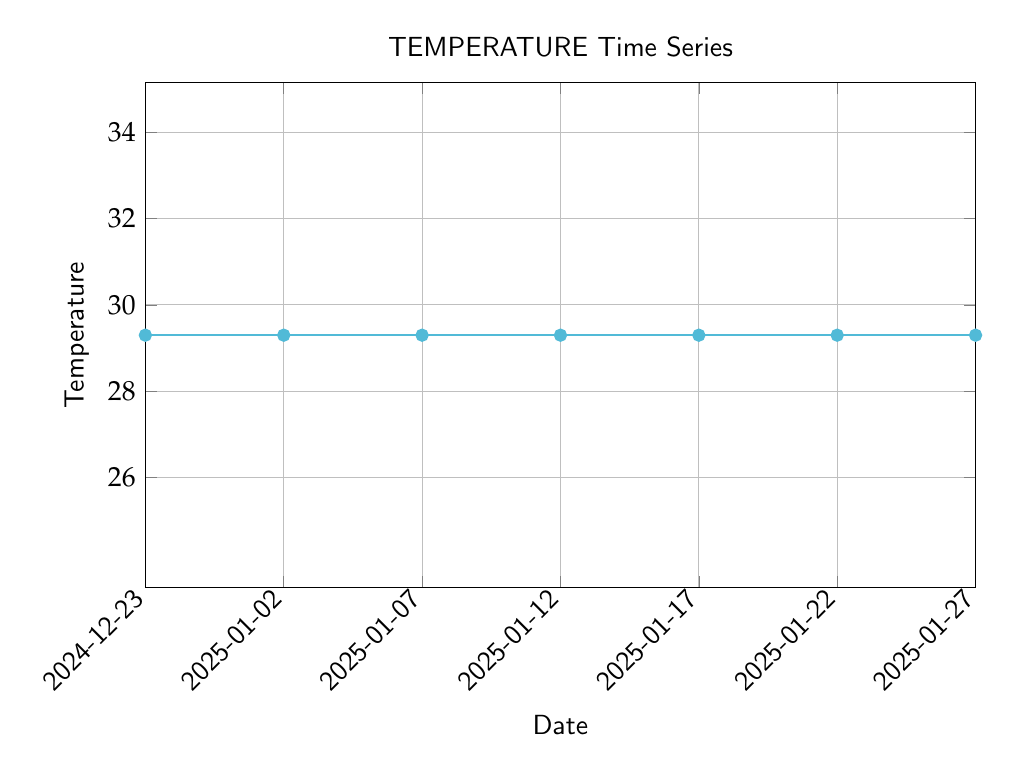
\begin{tikzpicture}
            \begin{axis}[
                width=\linewidth,
                height=8cm,
                xlabel={Date},
                ylabel={Temperature},
                xmin=1, xmax=7,
                % Use xtick=data to let pgfplots figure out ticks from xticklabels
                xtick=data,
                xticklabels={ % Use a join filter to ensure no trailing commas or extra spaces
                    2024-12-23, 2025-01-02, 2025-01-07, 2025-01-12, 2025-01-17, 2025-01-22, 2025-01-27
                },
                title={TEMPERATURE Time Series},
                grid=both,
                xticklabel style={rotate=45,anchor=east},
                enlargelimits=false,
                % Add "unbounded coords=jump" to handle potential non-numeric data gracefully
                unbounded coords=jump
            ]
            \addplot[
                color=hydrosenscyan,
                mark=*,
                thick,
            ]
            coordinates {
                % Safely generate coordinates on a single line
                    % Ensure y_val is numeric and not empty/None.
                    % If it could be missing, you might need a conditional check here
                    % e.g., 
                    (1, 29.295709228515648) % Use 'nan' for missing values
                    % Ensure y_val is numeric and not empty/None.
                    % If it could be missing, you might need a conditional check here
                    % e.g., 
                    (2, 29.295709228515648) % Use 'nan' for missing values
                    % Ensure y_val is numeric and not empty/None.
                    % If it could be missing, you might need a conditional check here
                    % e.g., 
                    (3, 29.295709228515648) % Use 'nan' for missing values
                    % Ensure y_val is numeric and not empty/None.
                    % If it could be missing, you might need a conditional check here
                    % e.g., 
                    (4, 29.295709228515648) % Use 'nan' for missing values
                    % Ensure y_val is numeric and not empty/None.
                    % If it could be missing, you might need a conditional check here
                    % e.g., 
                    (5, 29.295709228515648) % Use 'nan' for missing values
                    % Ensure y_val is numeric and not empty/None.
                    % If it could be missing, you might need a conditional check here
                    % e.g., 
                    (6, 29.295709228515648) % Use 'nan' for missing values
                    % Ensure y_val is numeric and not empty/None.
                    % If it could be missing, you might need a conditional check here
                    % e.g., 
                    (7, 29.295709228515648) % Use 'nan' for missing values
            };
            \end{axis}
            \end{tikzpicture}
        \end{center}
    \end{minipage}%
}\par % Keep this \par immediately after the closing brace of the \parbox
\vspace{1cm}


\newpage

\section*{CURVE NUMBER}
\textit{Runoff potential.}

\vspace{0.5cm}

\parbox{\textwidth}{ % Keep this parbox for horizontal layout
    \begin{minipage}[t]{0.48\textwidth}
        \vspace{0.3cm}
        \textbf{\Large{70.03}}
        \vspace{0.3cm}
        \textbf{MEAN VALUE}\\
        An average curve number of 70.03 indicates a moderate runoff potential in Name\_ABALOU Abla - Autre parcelle. This suggests that a moderate amount of rainfall would result in surface runoff.
        \vspace{0.5cm}

        \textbf{TIME SERIES INSIGHT}\\
        Curve number values fluctuated throughout the period, ranging from approximately 65.87 to 78.70. The variation suggests differences in runoff potential depending on short-term changes.
    \end{minipage}\hfill
    \begin{minipage}[t]{0.48\textwidth}
        \begin{center}
            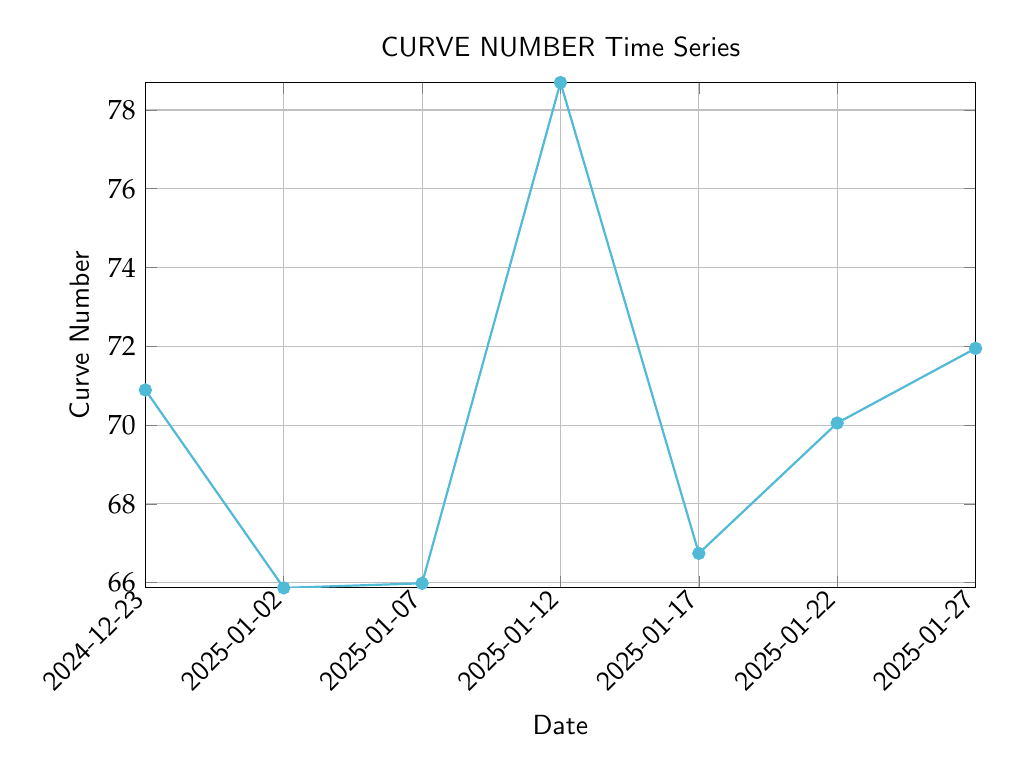
\begin{tikzpicture}
            \begin{axis}[
                width=\linewidth,
                height=8cm,
                xlabel={Date},
                ylabel={Curve Number},
                xmin=1, xmax=7,
                % Use xtick=data to let pgfplots figure out ticks from xticklabels
                xtick=data,
                xticklabels={ % Use a join filter to ensure no trailing commas or extra spaces
                    2024-12-23, 2025-01-02, 2025-01-07, 2025-01-12, 2025-01-17, 2025-01-22, 2025-01-27
                },
                title={CURVE NUMBER Time Series},
                grid=both,
                xticklabel style={rotate=45,anchor=east},
                enlargelimits=false,
                % Add "unbounded coords=jump" to handle potential non-numeric data gracefully
                unbounded coords=jump
            ]
            \addplot[
                color=hydrosenscyan,
                mark=*,
                thick,
            ]
            coordinates {
                % Safely generate coordinates on a single line
                    % Ensure y_val is numeric and not empty/None.
                    % If it could be missing, you might need a conditional check here
                    % e.g., 
                    (1, 70.89308553051583) % Use 'nan' for missing values
                    % Ensure y_val is numeric and not empty/None.
                    % If it could be missing, you might need a conditional check here
                    % e.g., 
                    (2, 65.86901523912354) % Use 'nan' for missing values
                    % Ensure y_val is numeric and not empty/None.
                    % If it could be missing, you might need a conditional check here
                    % e.g., 
                    (3, 65.98525540338092) % Use 'nan' for missing values
                    % Ensure y_val is numeric and not empty/None.
                    % If it could be missing, you might need a conditional check here
                    % e.g., 
                    (4, 78.69785637225098) % Use 'nan' for missing values
                    % Ensure y_val is numeric and not empty/None.
                    % If it could be missing, you might need a conditional check here
                    % e.g., 
                    (5, 66.74481216482332) % Use 'nan' for missing values
                    % Ensure y_val is numeric and not empty/None.
                    % If it could be missing, you might need a conditional check here
                    % e.g., 
                    (6, 70.05433968377068) % Use 'nan' for missing values
                    % Ensure y_val is numeric and not empty/None.
                    % If it could be missing, you might need a conditional check here
                    % e.g., 
                    (7, 71.94932288563587) % Use 'nan' for missing values
            };
            \end{axis}
            \end{tikzpicture}
        \end{center}
    \end{minipage}%
}\par % Keep this \par immediately after the closing brace of the \parbox
\vspace{1cm}


\newpage

% Action Plans Page
\section*{ACTION PLANS}

\begin{tcolorbox}[colback=white, colframe=hydrosenscyan]
Based on the data, the following actions are suggested:
\begin{itemize}
    \item \textbf{Implement efficient irrigation practices to address the lack of rainfall and ensure adequate water supply for vegetation.}
    \item \textbf{Monitor soil moisture levels regularly and adjust irrigation strategies as needed.}
    \item \textbf{Consider implementing soil conservation measures to minimize runoff potential and improve water infiltration.}
    \item \textbf{Select drought-resistant vegetation species for future plantings to reduce water demand.}
    \item \textbf{Conduct further investigation into the factors causing NDVI fluctuation and the runoff potential change.}
\end{itemize}
\end{tcolorbox}

\end{document}